%% =============================================================================
%% AI-Powered Project Management System with Automatic Task Prioritization
%% B.Tech Project Report — Department of CSE, Quantum University, Roorkee
%% =============================================================================
\documentclass[12pt,a4paper,oneside]{report}

%% ---------- Packages ---------------------------------------------------------
\usepackage[left=4cm, right=2cm, top=3cm, bottom=3cm]{geometry}
\usepackage{times}                       % Times New Roman
\usepackage{setspace}                    % 1.5 line spacing
\usepackage{graphicx}                    % Figures
\usepackage{float}                       % [H] placement
\usepackage{booktabs}                    % Professional tables
\usepackage{longtable}                   % Multi-page tables
\usepackage{array}                       % Column formatting
\usepackage{tabularx}                    % Full-width tables
\usepackage{caption}                     % Custom captions
\usepackage{subcaption}                  % Sub-figures
\usepackage{amsmath,amssymb}             % Mathematics
\usepackage{listings}                    % Code listings
\usepackage{xcolor}                      % Colors
\usepackage{hyperref}                    % Hyperlinks
\usepackage{url}                         % URL formatting
\usepackage{fancyhdr}                    % Headers/Footers
\usepackage{titlesec}                    % Section formatting
\usepackage{tocloft}                     % Table of contents formatting
\usepackage{enumitem}                    % List customisation
\usepackage{tikz}                        % Diagrams
\usetikzlibrary{shapes,arrows.meta,positioning,fit}

%% ---------- Page Style -------------------------------------------------------
\pagestyle{fancy}
\fancyhf{}
\fancyfoot[C]{\thepage}
\renewcommand{\headrulewidth}{0pt}

%% ---------- Spacing ----------------------------------------------------------
\onehalfspacing   % 1.5 line spacing as per guidelines

%% ---------- Section Formatting (14pt bold / 12pt bold) -----------------------
\titleformat{\chapter}[display]
  {\normalfont\large\bfseries\centering}
  {\MakeUppercase{\chaptertitlename}\ \thechapter}{12pt}{\Large\bfseries\MakeUppercase}
\titlespacing*{\chapter}{0pt}{-20pt}{20pt}

\titleformat{\section}
  {\normalfont\fontsize{14}{16}\bfseries}{\thesection}{1em}{}
\titlespacing*{\section}{0pt}{12pt}{6pt}

\titleformat{\subsection}
  {\normalfont\fontsize{12}{14}\bfseries}{\thesubsection}{1em}{}
\titlespacing*{\subsection}{0pt}{12pt}{6pt}

%% ---------- Code Listing Style -----------------------------------------------
\definecolor{codebg}{RGB}{248,248,248}
\definecolor{codegreen}{RGB}{34,139,34}
\definecolor{codegray}{RGB}{128,128,128}
\definecolor{codeblue}{RGB}{0,0,180}

\lstdefinestyle{codestyle}{
  backgroundcolor=\color{codebg},
  commentstyle=\color{codegreen},
  keywordstyle=\color{codeblue}\bfseries,
  numberstyle=\tiny\color{codegray},
  stringstyle=\color{red!70!black},
  basicstyle=\ttfamily\footnotesize,
  breaklines=true,
  captionpos=b,
  keepspaces=true,
  numbers=left,
  numbersep=5pt,
  showspaces=false,
  showstringspaces=false,
  tabsize=2,
  frame=single,
  rulecolor=\color{black!30},
}
\lstset{style=codestyle}

%% ---------- Hyperlink Setup --------------------------------------------------
\hypersetup{
  colorlinks=true,
  linkcolor=black,
  citecolor=blue!60!black,
  urlcolor=blue!60!black,
}

%% =============================================================================
%%                              DOCUMENT BEGIN
%% =============================================================================
\begin{document}

%% ======================== FRONT MATTER (Roman numerals) ======================
\pagenumbering{roman}

%% ---------- Title Page -------------------------------------------------------
\begin{titlepage}
\begin{center}

\vspace*{1cm}
{\large\textbf{AI-POWERED PROJECT MANAGEMENT SYSTEM\\WITH AUTOMATIC TASK PRIORITIZATION}}

\vspace{1.5cm}
{\normalsize Project report submitted in partial fulfillment of the requirement\\for the award of the Degree of B.\ Tech}

\vspace{1.5cm}
{\normalsize\textbf{Submitted by}}

\vspace{0.8cm}
\begin{tabular}{ll}
\textbf{Tushar Gautam}  & Roll No: 23030746 \\
\textbf{Uma Shankar}    & Roll No: 23030652 \\
\textbf{Likha Gummiku}  & Roll No: 23030846 \\
\textbf{Dipti Saini}    & Roll No: 23030565 \\
\end{tabular}

\vspace{1.5cm}
% University Logo — replace path with actual logo
% \includegraphics[width=3cm]{quantum_logo.png}

\vspace{0.5cm}
{\normalsize Department of Computer Science and Engineering\\
Quantum School of Technology\\
\textbf{Quantum University, Roorkee}\\
2026}

\end{center}
\end{titlepage}

%% ---------- Blank Page -------------------------------------------------------
\newpage\thispagestyle{empty}\mbox{}\newpage

%% ---------- Certificate ------------------------------------------------------
\newpage
\begin{center}
{\large\textbf{CERTIFICATE}}
\end{center}
\vspace{1cm}
\noindent
This is to certify that the project report entitled \textbf{``AI-Powered Project Management System with Automatic Task Prioritization''} being submitted by \textbf{Tushar Gautam} (23030746), \textbf{Uma Shankar} (23030652), \textbf{Likha Gummiku} (23030846), and \textbf{Dipti Saini} (23030565) in partial fulfillment for the award of the Degree of Bachelor of Technology in Computer Science and Engineering with specialization in Full Stack Development from the Department of Computer Science \& Engineering is a record of bonafide work carried out by them under my guidance and supervision.

\vspace{3cm}
\noindent
\begin{tabular}{p{6cm}p{6cm}}
\rule{5cm}{0.4pt} & \rule{5cm}{0.4pt} \\
(Name \& Signature)          & (Name \& Signature) \\
Project Guide                & Program Officer, CSE \\
\end{tabular}

\vspace{2.5cm}
\noindent
\begin{tabular}{p{6cm}}
\rule{5cm}{0.4pt} \\
(Name \& Signature) \\
HoD, CSE \& Dean Academics, QU \\
\end{tabular}
\thispagestyle{plain}

%% ---------- Declaration ------------------------------------------------------
\newpage
\begin{center}
{\large\textbf{DECLARATION}}
\end{center}
\vspace{1cm}
\noindent
We hereby declare that the project entitled \textbf{``AI-Powered Project Management System with Automatic Task Prioritization''} submitted for the B.\ Tech Degree in Computer Science and Engineering with specialization in Full Stack Development is our original work and the project has not formed the basis or submitted for the award of any degree, diploma, or any other similar titles in any other college/institute/university.

\vspace{2.5cm}
\noindent
\begin{tabular}{ll}
\textbf{Name:} & Tushar Gautam (23030746) \\
\textbf{Name:} & Uma Shankar (23030652) \\
\textbf{Name:} & Likha Gummiku (23030846) \\
\textbf{Name:} & Dipti Saini (23030565) \\
\end{tabular}

\vspace{1.5cm}
\noindent
\textbf{Place:} Roorkee\\
\textbf{Date:} \today
\thispagestyle{plain}

%% ---------- Acknowledgements -------------------------------------------------
\newpage
\begin{center}
{\large\textbf{ACKNOWLEDGEMENTS}}
\end{center}
\vspace{1cm}
\noindent
We would like to express our sincere gratitude to our project guide for their continuous guidance, encouragement, and valuable suggestions throughout the development of this project. Their constructive criticism and insightful feedback have been instrumental in shaping the direction of this work.

We are also thankful to the Head of the Department of Computer Science and Engineering, Quantum University, Roorkee, for providing the necessary facilities and an encouraging academic environment.

We extend our heartfelt thanks to all the faculty members of the Department of Computer Science and Engineering for their support and the knowledge they have imparted throughout our academic journey.

We would also like to thank our families and friends for their constant support and motivation during the course of this project.

Finally, we acknowledge the developers and contributors of the open-source tools, libraries, and frameworks that made this project possible, including React, Node.js, Express.js, MongoDB, and the numerous npm packages used in our implementation.
\thispagestyle{plain}

%% ---------- Abstract ---------------------------------------------------------
\newpage
\begin{center}
{\large\textbf{ABSTRACT}}
\end{center}
\vspace{1cm}
\noindent
Software development projects involve a large number of tasks that must be planned, assigned, monitored, and completed within limited time and resource constraints. As project size increases, project teams frequently face difficulty in determining which task should receive attention first. Conventional project management systems generally provide features for task creation, assignment, status tracking, deadlines, and workflow visualization; however, the actual prioritization of tasks often remains dependent on manual judgement.

This project presents the design, implementation, and evaluation of an \textbf{AI-Powered Project Management System with Automatic Task Prioritization}. The system integrates project planning, task management, Kanban-based workflow visualization, automatic task prioritization, AI-assisted task analysis, risk identification, and workload analysis within a unified web-based platform.

The central component is an \textbf{Automatic Task Prioritization Engine} that analyses five task-related factors --- deadline urgency (30\%), business impact (25\%), dependency impact (20\%), team workload (15\%), and task complexity (10\%) --- using a deterministic weighted scoring model to generate a measurable priority score between 0 and 100. The system also provides human-readable explanations showing why a particular task received its priority, thereby improving transparency and interpretability.

An \textbf{AI-assisted analysis layer} complements the deterministic priority engine by analysing task descriptions to suggest task complexity, estimated effort, required skills, possible risks, and smaller actionable subtasks. The AI layer uses a three-tier fallback architecture: a local rule-based engine (default), an optional local LLM via Ollama, and an optional external AI provider.

The system was developed using React 18, Vite, Tailwind CSS v4, Node.js, Express.js, MongoDB, and Mongoose. Testing was performed using Jest with 32 unit tests covering the priority engine, risk detection, configuration validation, and AI engine functionality. All tests passed successfully.

The proposed system successfully answers the core question: \textit{``What should the team work on next, and why?''}

\textbf{Keywords:} Project Management, Task Prioritization, Artificial Intelligence, Kanban, Decision Support System, Weighted Scoring Model, Full-Stack Web Application.
\thispagestyle{plain}

%% ---------- Table of Contents ------------------------------------------------
\newpage
\tableofcontents
\thispagestyle{plain}

%% ---------- List of Tables ---------------------------------------------------
\newpage
\listoftables
\thispagestyle{plain}

%% ---------- List of Figures --------------------------------------------------
\newpage
\listoffigures
\thispagestyle{plain}

%% ---------- List of Abbreviations -------------------------------------------
\newpage
\begin{center}
{\large\textbf{LIST OF ABBREVIATIONS}}
\end{center}
\vspace{1cm}
\begin{longtable}{p{3cm}p{10cm}}
\toprule
\textbf{Abbreviation} & \textbf{Full Form} \\
\midrule
AI     & Artificial Intelligence \\
API    & Application Programming Interface \\
CRUD   & Create, Read, Update, Delete \\
CSS    & Cascading Style Sheets \\
DB     & Database \\
DFD    & Data Flow Diagram \\
DOM    & Document Object Model \\
HTTP   & HyperText Transfer Protocol \\
JSON   & JavaScript Object Notation \\
JWT    & JSON Web Token \\
LLM    & Large Language Model \\
MERN   & MongoDB, Express, React, Node.js \\
NLP    & Natural Language Processing \\
ODM    & Object Document Mapper \\
PMIS   & Project Management Information System \\
REST   & Representational State Transfer \\
SBSE   & Search-Based Software Engineering \\
SPA    & Single Page Application \\
UI     & User Interface \\
UML    & Unified Modeling Language \\
UX     & User Experience \\
\bottomrule
\end{longtable}
\thispagestyle{plain}

%% ======================== MAIN MATTER (Arabic numerals) ======================
\newpage
\pagenumbering{arabic}

%% =============================================================================
%%                         CHAPTER 1: INTRODUCTION
%% =============================================================================
\chapter{Introduction}

\section{Background}

Project management is an essential activity in software development because the successful completion of a software product depends not only on programming but also on effective planning, organization, resource allocation, communication, monitoring, and decision making. A software project is normally divided into multiple activities or tasks that may involve different team members, deadlines, technical requirements, dependencies, levels of complexity, and business priorities. As a project progresses, the importance of individual tasks may change according to deadlines, completed dependencies, emerging risks, resource availability, and changes in project requirements.

In a small project, a project manager or development team can often prioritize tasks manually by considering experience and immediate requirements. However, manual decision making becomes more difficult as the number of tasks increases. A team may have several high-priority tasks, but not all of them can necessarily be executed simultaneously. Some tasks may have an approaching deadline, while another task may have a high business impact. A third task may block several other activities because it is a dependency. Similarly, a developer may already be assigned to multiple tasks, making workload an important consideration.

Traditional project management systems have addressed many aspects of this problem by providing centralized task repositories, dashboards, calendars, workflow boards, notifications, and reporting mechanisms. These systems improve visibility and coordination. However, the responsibility for deciding which task should be executed next may still remain with the project manager or individual team members.

\section{Task Prioritization in Software Development}

Task prioritization refers to the process of determining the relative order in which tasks should be addressed. It is closely related to requirements prioritization but is broader in the context of project execution because a task may represent a feature, bug fix, technical activity, testing activity, documentation task, infrastructure task, or other project activity.

Research has demonstrated that prioritization is a complex decision-making activity. Karlsson and Ryan proposed a cost-value approach in which requirements are evaluated according to their relative value and cost. Later systematic reviews further demonstrated that requirements prioritization has developed into a large research area containing numerous techniques and criteria.

\section{Importance of Multiple Criteria}

A software task can have different levels of importance depending on project context:

\begin{itemize}[noitemsep]
  \item \textbf{Deadline Urgency:} A task with a deadline approaching within a short period may need immediate attention.
  \item \textbf{Business Impact:} A task related to a core project feature, customer requirement, security issue, or important deliverable may have greater significance.
  \item \textbf{Dependencies:} If Task B cannot be completed until Task A is completed, then the status of Task A affects the overall project flow.
  \item \textbf{Team Workload:} A theoretically important task may not be immediately executable if the assigned developer is already overloaded.
  \item \textbf{Complexity:} A complex task may require more preparation, additional resources, or earlier initiation.
\end{itemize}

The proposed project combines these factors into a unified scoring mechanism.

\section{Artificial Intelligence in Project Management}

Artificial Intelligence has increasingly been investigated as a technology for supporting project management. Research reviews have identified applications of AI in project planning, scheduling, forecasting, risk management, performance monitoring, decision support, resource allocation, and uncertainty management.

For this reason, the proposed project separates AI-assisted analysis from the core prioritization calculation. The priority score is produced through a deterministic multi-factor model. AI assists in understanding task descriptions, suggesting subtasks, estimating complexity, identifying risks, and providing supporting recommendations.

\section{Problem Statement}

In software development projects, teams continuously manage tasks having different deadlines, business impacts, dependencies, complexities, estimated efforts, and resource requirements. Conventional project management systems provide facilities for task organization and workflow visualization, but the process of determining which task should receive attention first frequently depends on manual judgement.

Therefore, the problem addressed by this project is:

\begin{quote}
\textit{How can a project management system automatically analyse multiple task and project factors to generate an explainable task-priority recommendation while providing AI-assisted support for task understanding, task breakdown, risk identification, and project decision making?}
\end{quote}

\section{Objectives}

The following objectives have been defined for the proposed project:

\begin{enumerate}[noitemsep]
  \item To develop a full-stack web-based project management system with user authentication, project management, and task management capabilities.
  \item To implement a Kanban-based workflow visualization for task status tracking across five stages: Backlog, To Do, In Progress, In Review, and Done.
  \item To design and implement an automatic task prioritization engine using a deterministic weighted scoring model that considers deadline urgency, business impact, dependency impact, team workload, and task complexity.
  \item To generate human-readable priority explanations that describe why a task received its priority score.
  \item To implement an AI-assisted task analysis layer capable of analysing task descriptions, estimating complexity, suggesting required skills, identifying risks, and generating subtask breakdowns.
  \item To implement risk detection based on project and task factors.
  \item To implement team workload analysis based on task assignments.
  \item To provide project analytics and dashboard visualizations.
  \item To test the system using unit tests to verify priority engine accuracy and AI engine functionality.
  \item To document the system for academic evaluation and demonstration.
\end{enumerate}

\section{Scope and Limitations}

\subsection{Scope}
The system focuses on software project management with the minimum functional scope including user authentication, project creation, team management, task management, task assignment, deadlines, dependencies, Kanban workflow, automatic priority calculation, priority explanations, AI-assisted task analysis, risk indicators, workload analysis, and basic project analytics.

\subsection{Limitations}
\begin{itemize}[noitemsep]
  \item No real-time collaboration (WebSocket).
  \item No email or push notifications.
  \item No sprint management or velocity tracking.
  \item No file attachments.
  \item The local AI engine uses rule-based pattern matching, not a trained machine learning model.
  \item Single-instance deployment (no horizontal scaling).
\end{itemize}

\section{Organization of Report}

The remaining chapters of this report are organized as follows:
\begin{itemize}[noitemsep]
  \item \textbf{Chapter 2} presents the literature survey covering requirements prioritization, task prioritization, Kanban, and AI in project management.
  \item \textbf{Chapter 3} describes the proposed methodology, system architecture, and design decisions.
  \item \textbf{Chapter 4} presents the system design including database design, UML diagrams, and component architecture.
  \item \textbf{Chapter 5} describes the implementation details including priority engine, AI engine, and frontend components.
  \item \textbf{Chapter 6} presents the results, output screens, and testing.
  \item \textbf{Chapter 7} presents conclusions.
  \item \textbf{Chapter 8} discusses future work and recommendations.
\end{itemize}


%% =============================================================================
%%                      CHAPTER 2: LITERATURE SURVEY
%% =============================================================================
\chapter{Literature Survey}

\section{Introduction}

The literature survey for this project focuses on five closely related research areas: (1) software requirements prioritization, (2) software task and issue prioritization, (3) Agile and Kanban-based project management, (4) Artificial Intelligence in project management, and (5) Project Management Information Systems and AI-assisted decision support.

\section{Review of Existing Research}

The following table summarizes relevant research studies that informed the design of the proposed system.

\begin{longtable}{|c|p{3.5cm}|p{3.5cm}|p{5cm}|}
\caption{Literature Review of Relevant Research Studies} \label{tab:litreview} \\
\hline
\textbf{No.} & \textbf{Study} & \textbf{Research Focus} & \textbf{Major Findings and Relevance} \\
\hline
\endfirsthead
\hline
\textbf{No.} & \textbf{Study} & \textbf{Research Focus} & \textbf{Major Findings and Relevance} \\
\hline
\endhead
\hline
\endfoot
1 & Karlsson and Ryan (1997) & Cost-value approach for software requirements prioritization & Demonstrated that prioritization can be treated as a structured decision problem using multiple measurable factors. \\
\hline
2 & Karlsson, Wohlin and Regnell (1998) & Evaluation of six requirements prioritization methods & Compared several methods and identified scalability concerns, motivating a lightweight scoring mechanism. \\
\hline
3 & Achimugu et al. (2014) & Systematic literature review of requirements prioritization & Identified issues including scalability, changing requirements, and dependency management. \\
\hline
4 & Ahmad et al. (2018) & Systematic mapping of Kanban in software engineering & Analysed Kanban literature and identified benefits, challenges, and research opportunities. \\
\hline
5 & Jarz\k{e}bowicz and Sitko (2020) & Industrial survey of Agile requirements prioritization & Found business value to be common while complexity and interdependencies were also considered. \\
\hline
6 & Bukhsh, Bukhsh and Daneva (2020) & Systematic review of requirements prioritization & Reviewed 102 papers; found increasing use of fuzzy logic, optimization, and machine learning. \\
\hline
7 & Bento et al. (2022) & Systematic review of AI in project management & Identified increasing interest in AI for project management decision-support. \\
\hline
8 & Bugayenko et al. (2023) & Systematic review of task prioritization in software development & Found that much research focuses on bugs and issues; motivates broader task-level prioritization. \\
\hline
9 & Taboada et al. (2023) & Systematic review of AI-enabled project management & Identified opportunities for planning, forecasting, and decision support using AI. \\
\hline
10 & Nenni et al. (2025) & Systematic review of AI and project management & Reviewed 215 papers; examined AI applications in risk management and decision support. \\
\hline
\end{longtable}

\section{Identified Research Gap}

The literature reveals the following gaps:
\begin{enumerate}[noitemsep]
  \item Existing requirements prioritization methods frequently focus on requirements selection or release planning rather than continuous task-level prioritization.
  \item Existing software task prioritization research often concentrates on specialized categories such as bugs, issues, and pull requests.
  \item Kanban systems provide workflow visualization but do not inherently provide multi-factor automatic task prioritization.
  \item AI project management research demonstrates strong potential but identifies challenges related to transparency, integration, and validation.
\end{enumerate}

The proposed system addresses this gap through an integrated pipeline: Task and Project Data $\rightarrow$ Multi-Factor Analysis $\rightarrow$ Automatic Priority Score $\rightarrow$ Explainable Recommendation $\rightarrow$ Kanban Decision Support.


%% =============================================================================
%%                       CHAPTER 3: METHODOLOGY
%% =============================================================================
\chapter{Methodology}

\section{Development Methodology}

The system follows an iterative Agile software development methodology. Development was performed incrementally across twelve phases:

\begin{enumerate}[noitemsep]
  \item Project scaffold and environment setup
  \item Database models and schema design
  \item User authentication and authorization
  \item Project management API
  \item Task management API
  \item Priority engine development
  \item AI engine development
  \item Controllers and route integration
  \item Seed data creation
  \item Frontend development
  \item Testing
  \item Documentation
\end{enumerate}

\section{Technology Stack}

\begin{table}[H]
\centering
\caption{Technology Stack}
\label{tab:techstack}
\begin{tabular}{|l|l|}
\hline
\textbf{Layer}      & \textbf{Technology} \\
\hline
Frontend            & React 18, Vite, Tailwind CSS v4, React Router v6, Recharts \\
\hline
Backend             & Node.js, Express.js, Mongoose, JWT, bcrypt \\
\hline
Database            & MongoDB 8.x \\
\hline
AI Engine           & Local rule-based intelligence engine \\
\hline
Drag \& Drop        & @hello-pangea/dnd \\
\hline
Testing             & Jest \\
\hline
\end{tabular}
\end{table}

\section{System Architecture}

The application uses a modular client-server architecture consisting of three main layers:

\begin{figure}[H]
\centering
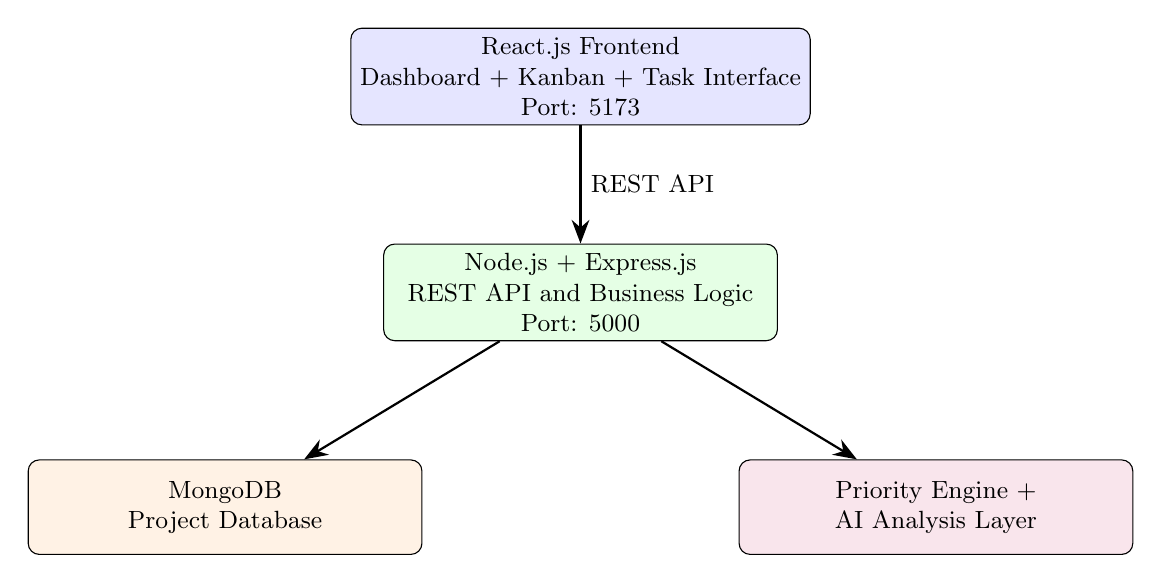
\begin{tikzpicture}[
  box/.style={draw, rounded corners, minimum width=5cm, minimum height=1.2cm, align=center, font=\small},
  arrow/.style={-{Stealth[length=3mm]}, thick}
]
\node[box, fill=blue!10] (frontend) {React.js Frontend\\Dashboard + Kanban + Task Interface\\Port: 5173};
\node[box, fill=green!10, below=1.5cm of frontend] (backend) {Node.js + Express.js\\REST API and Business Logic\\Port: 5000};
\node[box, fill=orange!10, below left=1.5cm and -0.5cm of backend] (db) {MongoDB\\Project Database};
\node[box, fill=purple!10, below right=1.5cm and -0.5cm of backend] (ai) {Priority Engine +\\AI Analysis Layer};

\draw[arrow] (frontend) -- node[right, font=\small] {REST API} (backend);
\draw[arrow] (backend) -- (db);
\draw[arrow] (backend) -- (ai);
\end{tikzpicture}
\caption{System Architecture Diagram}
\label{fig:architecture}
\end{figure}

\section{Priority Algorithm}

The automatic task prioritization uses a deterministic weighted scoring formula:

\begin{equation}
\text{Priority Score} = 0.30 \times U + 0.25 \times B + 0.20 \times D + 0.15 \times W + 0.10 \times C
\label{eq:priority}
\end{equation}

Where:
\begin{itemize}[noitemsep]
  \item $U$ = Deadline Urgency (0--100)
  \item $B$ = Business Impact (0--100)
  \item $D$ = Dependency Impact (0--100)
  \item $W$ = Team Workload (0--100)
  \item $C$ = Task Complexity (0--100)
\end{itemize}

All factors are normalized to the range 0--100. The final score is also in the range 0--100.

\begin{table}[H]
\centering
\caption{Priority Score Categories}
\label{tab:categories}
\begin{tabular}{|l|l|}
\hline
\textbf{Score Range} & \textbf{Category} \\
\hline
0--30     & LOW \\
31--60    & MEDIUM \\
61--80    & HIGH \\
81--100   & CRITICAL \\
\hline
\end{tabular}
\end{table}

\subsection{Deadline Urgency Calculation}

The deadline urgency is calculated based on the number of days remaining until the task deadline:

\begin{table}[H]
\centering
\caption{Deadline Urgency Scoring}
\label{tab:deadline}
\begin{tabular}{|l|c|}
\hline
\textbf{Days Remaining} & \textbf{Urgency Score} \\
\hline
Past deadline or $\leq$ 1 day  & 100 \\
2--3 days                      & 90  \\
4--7 days                      & 75  \\
8--14 days                     & 55  \\
15--30 days                    & 35  \\
$>$ 30 days or no deadline     & 20  \\
\hline
\end{tabular}
\end{table}

\subsection{Risk Detection}

The system implements deterministic risk detection based on six factors:
\begin{enumerate}[noitemsep]
  \item Deadline has passed
  \item Deadline approaching (within 3 days)
  \item High complexity task
  \item No developer assigned
  \item Multiple dependencies ($\geq$ 3)
  \item Large estimated effort ($\geq$ 20 hours)
\end{enumerate}

Risk levels are assigned as: LOW (0--1 factors), MEDIUM (2 factors), HIGH (3--4 factors), CRITICAL (5+ factors).


%% =============================================================================
%%                       CHAPTER 4: SYSTEM DESIGN
%% =============================================================================
\chapter{System Design}

\section{Database Design}

The system uses MongoDB with Mongoose ODM. Five collections are defined:

\begin{table}[H]
\centering
\caption{Database Collections}
\label{tab:collections}
\begin{tabular}{|l|p{9cm}|}
\hline
\textbf{Collection} & \textbf{Key Fields} \\
\hline
Users       & name, email, passwordHash, role, skills \\
\hline
Projects    & name, description, owner, members, startDate, endDate, status \\
\hline
Tasks       & title, description, project, assignedTo, deadline, status, priority, businessImpact, complexity, estimatedHours, dependencies, priorityScore, riskLevel, aiAnalysis \\
\hline
Activities  & user, project, task, action, details \\
\hline
AiAnalyses  & task, provider, analysis, breakdown, explanation \\
\hline
\end{tabular}
\end{table}

\section{Use Case Diagram}

\begin{figure}[H]
\centering
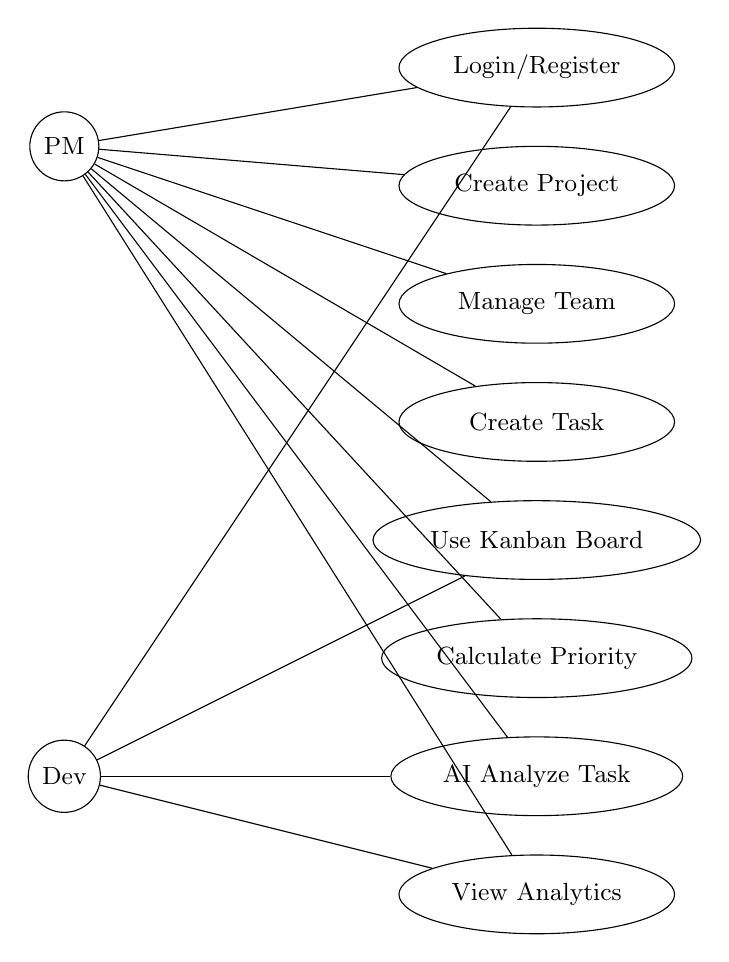
\begin{tikzpicture}[
  actor/.style={circle, draw, minimum size=0.8cm, font=\small},
  usecase/.style={ellipse, draw, minimum width=3.5cm, minimum height=1cm, align=center, font=\small},
]
\node[actor] (pm) at (0,0) {PM};
\node[actor] (dev) at (0,-8) {Dev};

\node[usecase] (login) at (6,1) {Login/Register};
\node[usecase] (createproj) at (6,-0.5) {Create Project};
\node[usecase] (manageteam) at (6,-2) {Manage Team};
\node[usecase] (createtask) at (6,-3.5) {Create Task};
\node[usecase] (kanban) at (6,-5) {Use Kanban Board};
\node[usecase] (calcpri) at (6,-6.5) {Calculate Priority};
\node[usecase] (aianalyze) at (6,-8) {AI Analyze Task};
\node[usecase] (analytics) at (6,-9.5) {View Analytics};

\draw (pm) -- (login);
\draw (pm) -- (createproj);
\draw (pm) -- (manageteam);
\draw (pm) -- (createtask);
\draw (pm) -- (kanban);
\draw (pm) -- (calcpri);
\draw (pm) -- (aianalyze);
\draw (pm) -- (analytics);

\draw (dev) -- (login);
\draw (dev) -- (kanban);
\draw (dev) -- (aianalyze);
\draw (dev) -- (analytics);
\end{tikzpicture}
\caption{Use Case Diagram}
\label{fig:usecase}
\end{figure}

\section{Class Diagram}

\begin{figure}[H]
\centering
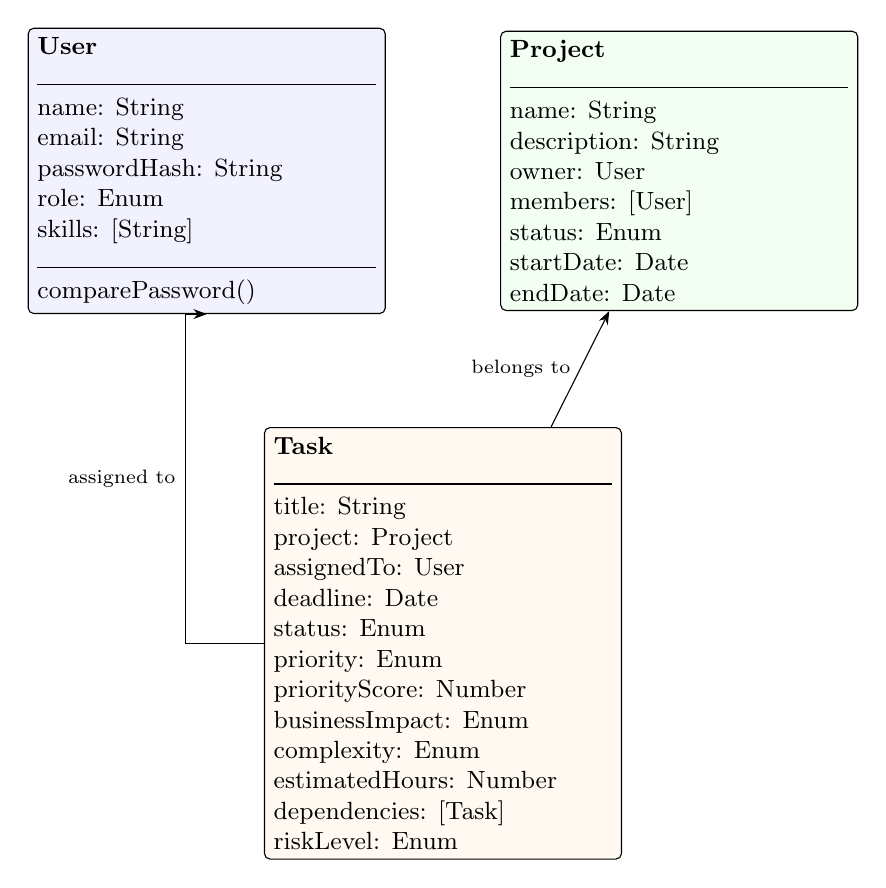
\begin{tikzpicture}[
  class/.style={draw, rectangle, rounded corners=2pt, minimum width=4.5cm, font=\small, align=left},
]
\node[class, fill=blue!5] (user) at (0,0) {
  \textbf{User}\\
  \rule{4.3cm}{0.4pt}\\
  name: String\\
  email: String\\
  passwordHash: String\\
  role: Enum\\
  skills: [String]\\
  \rule{4.3cm}{0.4pt}\\
  comparePassword()
};

\node[class, fill=green!5] (project) at (6,0) {
  \textbf{Project}\\
  \rule{4.3cm}{0.4pt}\\
  name: String\\
  description: String\\
  owner: User\\
  members: [User]\\
  status: Enum\\
  startDate: Date\\
  endDate: Date
};

\node[class, fill=orange!5] (task) at (3,-6) {
  \textbf{Task}\\
  \rule{4.3cm}{0.4pt}\\
  title: String\\
  project: Project\\
  assignedTo: User\\
  deadline: Date\\
  status: Enum\\
  priority: Enum\\
  priorityScore: Number\\
  businessImpact: Enum\\
  complexity: Enum\\
  estimatedHours: Number\\
  dependencies: [Task]\\
  riskLevel: Enum
};

\draw[-{Stealth}] (task) -- node[left, font=\scriptsize] {belongs to} (project);
\draw[-{Stealth}] (task.west) -- ++(-1,0) |- node[left, font=\scriptsize, near start] {assigned to} (user.south);
\end{tikzpicture}
\caption{Class Diagram (Simplified)}
\label{fig:classdiagram}
\end{figure}

\section{Data Flow Diagram}

\subsection{Level 0 DFD (Context Diagram)}

\begin{figure}[H]
\centering
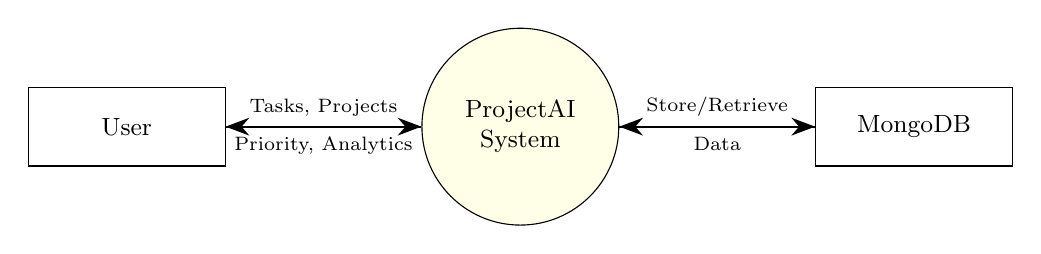
\begin{tikzpicture}[
  entity/.style={rectangle, draw, minimum width=2.5cm, minimum height=1cm, font=\small},
  process/.style={circle, draw, minimum size=2.5cm, font=\small, align=center},
  arrow/.style={-{Stealth[length=3mm]}, thick}
]
\node[entity] (user) at (-5,0) {User};
\node[process, fill=yellow!10] (system) at (0,0) {ProjectAI\\System};
\node[entity] (db) at (5,0) {MongoDB};

\draw[arrow] (user) -- node[above, font=\scriptsize] {Tasks, Projects} (system);
\draw[arrow] (system) -- node[above, font=\scriptsize] {Store/Retrieve} (db);
\draw[arrow, dashed] (system) -- node[below, font=\scriptsize] {Priority, Analytics} (user);
\draw[arrow, dashed] (db) -- node[below, font=\scriptsize] {Data} (system);
\end{tikzpicture}
\caption{Level 0 DFD -- Context Diagram}
\label{fig:dfd0}
\end{figure}

\section{Sequence Diagram: Priority Calculation}

\begin{figure}[H]
\centering
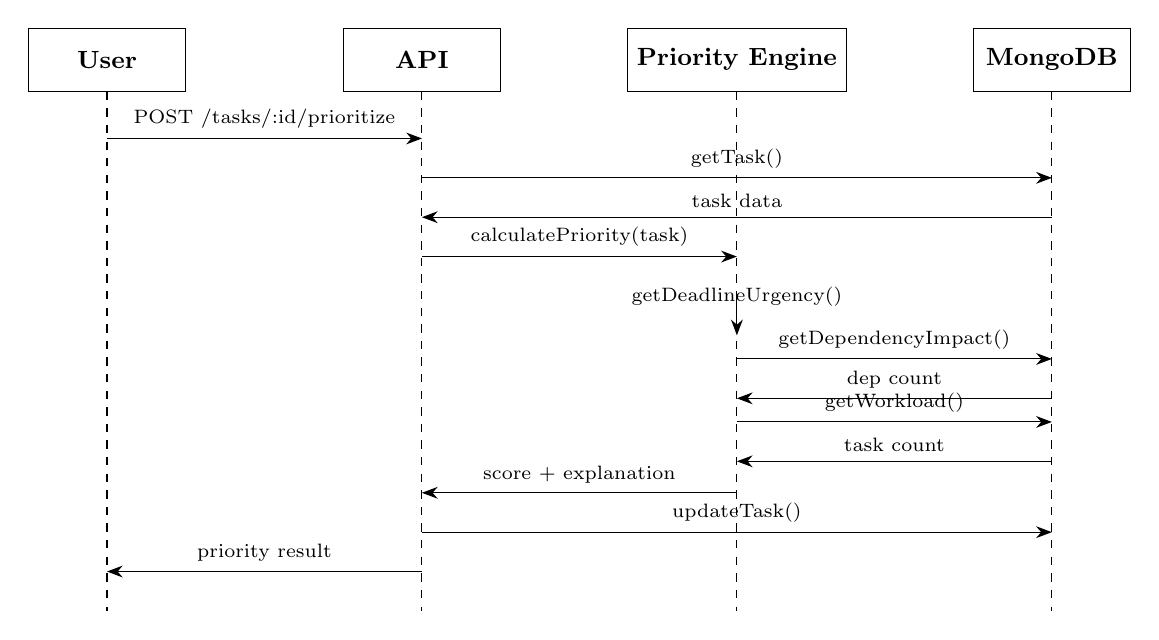
\begin{tikzpicture}[
  obj/.style={rectangle, draw, minimum width=2cm, minimum height=0.8cm, font=\small\bfseries},
  msg/.style={-{Stealth[length=2mm]}, font=\scriptsize},
]
\node[obj] (user) at (0,0) {User};
\node[obj] (api) at (4,0) {API};
\node[obj] (pri) at (8,0) {Priority Engine};
\node[obj] (db) at (12,0) {MongoDB};

\draw[dashed] (user) -- (0,-7);
\draw[dashed] (api) -- (4,-7);
\draw[dashed] (pri) -- (8,-7);
\draw[dashed] (db) -- (12,-7);

\draw[msg] (0,-1) -- node[above] {POST /tasks/:id/prioritize} (4,-1);
\draw[msg] (4,-1.5) -- node[above] {getTask()} (12,-1.5);
\draw[msg] (12,-2) -- node[above] {task data} (4,-2);
\draw[msg] (4,-2.5) -- node[above] {calculatePriority(task)} (8,-2.5);
\draw[msg] (8,-3) -- node[above] {getDeadlineUrgency()} (8,-3.5);
\draw[msg] (8,-3.8) -- node[above] {getDependencyImpact()} (12,-3.8);
\draw[msg] (12,-4.3) -- node[above] {dep count} (8,-4.3);
\draw[msg] (8,-4.6) -- node[above] {getWorkload()} (12,-4.6);
\draw[msg] (12,-5.1) -- node[above] {task count} (8,-5.1);
\draw[msg] (8,-5.5) -- node[above] {score + explanation} (4,-5.5);
\draw[msg] (4,-6) -- node[above] {updateTask()} (12,-6);
\draw[msg] (4,-6.5) -- node[above] {priority result} (0,-6.5);
\end{tikzpicture}
\caption{Sequence Diagram -- Priority Calculation}
\label{fig:sequence}
\end{figure}


%% =============================================================================
%%                     CHAPTER 5: IMPLEMENTATION
%% =============================================================================
\chapter{Implementation}

\section{Project Structure}

\begin{lstlisting}[language={}, caption={Project Directory Structure}]
project-management-ai/
+-- client/                  # React + Vite Frontend
|   +-- src/
|   |   +-- components/      # Reusable UI components
|   |   +-- context/         # Auth context
|   |   +-- layouts/         # App layout
|   |   +-- pages/           # Route pages (8)
|   |   +-- services/        # API service layer
|   |   +-- utils/           # Helpers, constants
+-- server/                  # Node.js + Express Backend
|   +-- src/
|   |   +-- config/          # DB, priority weights, AI config
|   |   +-- controllers/     # Route handlers (5)
|   |   +-- middleware/       # Auth, error handling
|   |   +-- models/          # Mongoose schemas (5)
|   |   +-- routes/          # Express routes (6)
|   |   +-- services/
|   |   |   +-- ai/          # AI service layer (3)
|   |   |   +-- priority/    # Priority engine (5)
|   |   +-- utils/           # Seed script
|   +-- tests/               # Jest unit tests
+-- README.md
\end{lstlisting}

\section{Priority Engine Implementation}

The priority engine consists of five service modules:

\subsection{Deadline Service}

Calculates urgency based on the number of days remaining until the task deadline. Past deadlines receive a score of 100. Tasks with no deadline receive a minimum score of 20.

\subsection{Dependency Service}

Queries the database to count the number of tasks that depend on the current task (downstream dependencies). The dependency impact score is calculated as:

\begin{equation}
D = \min(20 + (\text{downstream count} \times 20),\ 100)
\end{equation}

\subsection{Workload Service}

Queries the database to count the number of active tasks assigned to the same developer. The workload score is inversely proportional to the available developer capacity.

\subsection{Risk Service}

Evaluates six risk factors and assigns a composite risk level. Each identified factor contributes to the risk score. The factors are: overdue deadline, approaching deadline, high complexity, unassigned developer, multiple dependencies, and large effort estimate.

\subsection{Priority Orchestrator}

Combines all factor scores using the weighted formula (Equation~\ref{eq:priority}), assigns a priority category, generates a human-readable explanation, and persists the result to the database.

\section{AI Engine Implementation}

The AI engine uses a three-tier fallback architecture:

\begin{enumerate}[noitemsep]
  \item \textbf{Local Rule-Based Engine (Default):} Uses 50+ keyword patterns for skill detection, template-based subtask generation for common task types (authentication, CRUD, payment, dashboard), and deterministic complexity estimation.
  \item \textbf{Ollama Integration (Optional):} Connects to a locally installed Ollama LLM instance for natural language task analysis.
  \item \textbf{External AI Provider (Future):} Placeholder for external API integration.
\end{enumerate}

\section{Frontend Implementation}

The frontend is built with React 18 and Vite, using Tailwind CSS v4 for styling. Key pages include:

\begin{itemize}[noitemsep]
  \item \textbf{Dashboard:} Displays AI-recommended next tasks, statistics cards, activity feed, and priority distribution chart.
  \item \textbf{Kanban Board:} Five-column drag-and-drop board using @hello-pangea/dnd. Tasks are sorted by priority score within each column.
  \item \textbf{AI Assistant:} Standalone page for task analysis and breakdown.
  \item \textbf{Analytics:} Recharts-based bar and pie charts for task status, priority, and risk distribution.
  \item \textbf{Team:} Workload visualization per developer.
\end{itemize}

\section{API Endpoints}

\begin{table}[H]
\centering
\caption{REST API Endpoints}
\label{tab:api}
\begin{tabular}{|l|l|l|p{4.5cm}|}
\hline
\textbf{Method} & \textbf{Endpoint} & \textbf{Auth} & \textbf{Description} \\
\hline
POST & /api/auth/register & No & Register user \\
POST & /api/auth/login & No & Login \\
GET  & /api/auth/me & Yes & Current user \\
GET  & /api/projects & Yes & List projects \\
POST & /api/projects & PM & Create project \\
GET  & /api/tasks & Yes & List tasks \\
POST & /api/tasks & PM & Create task \\
POST & /api/tasks/:id/prioritize & PM & Calculate priority \\
POST & /api/ai/analyze-task & Yes & AI task analysis \\
POST & /api/ai/breakdown-task & Yes & AI task breakdown \\
GET  & /api/analytics/dashboard & Yes & Dashboard stats \\
GET  & /api/analytics/workload & Yes & Team workload \\
\hline
\end{tabular}
\end{table}

\section{Security Implementation}

\begin{itemize}[noitemsep]
  \item Passwords hashed using bcrypt with 12 salt rounds.
  \item JWT-based authentication with configurable expiry.
  \item Role-based access control (Project Manager, Developer, Viewer).
  \item Password never returned in API responses (\texttt{select: false}).
  \item CORS configured for frontend origin.
  \item Environment variables for secrets.
\end{itemize}


%% =============================================================================
%%                  CHAPTER 6: RESULTS AND DISCUSSIONS
%% =============================================================================
\chapter{Results and Discussions}

\section{Testing Results}

The system was tested using Jest with 32 unit tests covering the priority engine, risk detection, configuration validation, and AI engine. All tests passed successfully.

\begin{table}[H]
\centering
\caption{Unit Test Results}
\label{tab:tests}
\begin{tabular}{|l|c|c|}
\hline
\textbf{Test Suite} & \textbf{Tests} & \textbf{Status} \\
\hline
Deadline Urgency Calculator   & 10 & All Passed \\
Priority Weights Configuration & 3  & All Passed \\
Business Impact Mapping        & 4  & All Passed \\
Complexity Mapping             & 3  & All Passed \\
Priority Score Calculation     & 3  & All Passed \\
Risk Detection                 & 4  & All Passed \\
Local AI Engine                & 5  & All Passed \\
\hline
\textbf{Total}                & \textbf{32} & \textbf{All Passed} \\
\hline
\end{tabular}
\end{table}

\section{Build Verification}

\begin{table}[H]
\centering
\caption{Build Verification Results}
\label{tab:build}
\begin{tabular}{|l|l|}
\hline
\textbf{Metric} & \textbf{Result} \\
\hline
Modules Transformed & 669 \\
Build Errors & 0 \\
CSS Bundle Size & 22.60 KB (5.17 KB gzipped) \\
JS Bundle Size & 840.41 KB (251.15 KB gzipped) \\
Build Time & 7.10 seconds \\
\hline
\end{tabular}
\end{table}

\section{Priority Calculation Verification}

\begin{table}[H]
\centering
\caption{Sample Priority Calculation}
\label{tab:pricalc}
\begin{tabular}{|l|c|c|c|}
\hline
\textbf{Factor} & \textbf{Weight} & \textbf{Score} & \textbf{Weighted} \\
\hline
Urgency           & 0.30 & 90  & 27.0 \\
Business Impact   & 0.25 & 100 & 25.0 \\
Dependency Impact & 0.20 & 80  & 16.0 \\
Workload          & 0.15 & 60  & 9.0  \\
Complexity        & 0.10 & 90  & 9.0  \\
\hline
\textbf{Total}    &      &     & \textbf{86.0 (CRITICAL)} \\
\hline
\end{tabular}
\end{table}

\section{Output Screens}

% Note: Replace these with actual screenshot images
% \begin{figure}[H]
% \centering
% \includegraphics[width=\textwidth]{screenshots/login.png}
% \caption{Login Page}
% \label{fig:login}
% \end{figure}

% \begin{figure}[H]
% \centering
% \includegraphics[width=\textwidth]{screenshots/dashboard.png}
% \caption{Dashboard with AI Recommended Tasks}
% \label{fig:dashboard}
% \end{figure}

% \begin{figure}[H]
% \centering
% \includegraphics[width=\textwidth]{screenshots/kanban.png}
% \caption{Kanban Board with Priority-Sorted Tasks}
% \label{fig:kanban}
% \end{figure}

% \begin{figure}[H]
% \centering
% \includegraphics[width=\textwidth]{screenshots/ai_assistant.png}
% \caption{AI Assistant -- Task Analysis and Breakdown}
% \label{fig:aiassistant}
% \end{figure}

\textit{Note: Screenshots of Login Page, Dashboard, Kanban Board, AI Assistant, Analytics, and Team pages should be included here. Use the application at http://localhost:5174 to capture screenshots.}


%% =============================================================================
%%                       CHAPTER 7: CONCLUSION
%% =============================================================================
\chapter{Conclusion}

The project successfully designed, implemented, and tested an AI-Powered Project Management System with Automatic Task Prioritization. The system addresses the core problem: ``What should the team work on next, and why?''

The key contributions of this project are:

\begin{enumerate}[noitemsep]
  \item A \textbf{deterministic priority scoring engine} that analyses five task-related factors using a weighted formula to produce a measurable, reproducible priority score.
  \item \textbf{Human-readable priority explanations} that describe the factors contributing to each task's priority, improving transparency and interpretability.
  \item An \textbf{AI-assisted task analysis layer} with a three-tier fallback architecture that provides complexity estimation, skill detection, risk identification, and subtask generation without requiring external API keys or heavy infrastructure.
  \item \textbf{Deterministic risk detection} based on six project factors, enabling early identification of at-risk tasks.
  \item A \textbf{Kanban-based workflow} with drag-and-drop functionality and priority-aware task ordering.
  \item A \textbf{comprehensive analytics dashboard} with real-time statistics and visualizations.
  \item A \textbf{modular, local-first architecture} that runs entirely on a single machine without cloud dependencies, Docker, or paid APIs.
\end{enumerate}

The system was validated through 32 unit tests (all passing), a successful production build (669 modules, 0 errors), and live demonstration with seed data comprising 4 users, 1 project, and 10 tasks.


%% =============================================================================
%%                       CHAPTER 8: FUTURE WORK
%% =============================================================================
\chapter{Future Work}

The following enhancements are recommended for future development:

\begin{enumerate}[noitemsep]
  \item \textbf{Sprint Management:} Implement sprint planning, velocity tracking, and burndown charts.
  \item \textbf{Real-Time Collaboration:} Add WebSocket-based real-time updates for team collaboration.
  \item \textbf{Email/Push Notifications:} Notify team members about deadline changes, task assignments, and priority updates.
  \item \textbf{GitHub Integration:} Link tasks to commits, branches, and pull requests.
  \item \textbf{Predictive Analytics:} Use historical project data to predict task completion times and project delivery estimates.
  \item \textbf{ML-Based Priority Prediction:} Train a machine learning model on historical priority decisions to provide data-driven priority suggestions.
  \item \textbf{Mobile-Responsive PWA:} Convert the application into a Progressive Web App for mobile access.
  \item \textbf{CI/CD Pipeline Integration:} Integrate with Jenkins, GitHub Actions, or GitLab CI for automated testing and deployment.
  \item \textbf{Advanced AI Models:} Integrate with larger language models for more sophisticated task analysis and natural language query support.
  \item \textbf{Multi-Project Portfolio Management:} Support managing multiple projects simultaneously with cross-project analytics.
\end{enumerate}


%% =============================================================================
%%                        REFERENCES / BIBLIOGRAPHY
%% =============================================================================
\begin{thebibliography}{99}

\bibitem{karlsson1997}
Karlsson, J. and Ryan, K. (1997). A cost-value approach for prioritizing requirements. \textit{IEEE Software}, 14(5), 67--74.

\bibitem{karlsson1998}
Karlsson, J., Wohlin, C. and Regnell, B. (1998). An evaluation of methods for prioritizing software requirements. \textit{Information and Software Technology}, 39(14--15), 939--947.

\bibitem{kukreja2013}
Kukreja, N., Payyavula, S.S., Boehm, B. and Padmanabhuni, S. (2013). Value-based requirements prioritization: Usage experiences. \textit{Procedia Computer Science}, 16, 806--813.

\bibitem{achimugu2014}
Achimugu, P., Selamat, A., Ibrahim, R. and Mahrin, M.N.R. (2014). A systematic literature review of software requirements prioritization research. \textit{Information and Software Technology}, 56(6), 568--585.

\bibitem{sher2014}
Sher, F., Jawawi, D.N.A., Mohamad, R. and Babar, M.I. (2014). Requirements prioritization techniques and different aspects for prioritization. In \textit{2014 8th Malaysian Software Engineering Conference (MySEC)}, IEEE, 187--192.

\bibitem{pitangueira2015}
Pitangueira, A.M., Maciel, R.S.P. and Barros, M. (2015). Software requirements selection and prioritization using SBSE approaches: A systematic review and mapping of the literature. \textit{Journal of Systems and Software}, 103, 267--280.

\bibitem{vanderveen2015}
van der Veen, E., Gousios, G. and Zaidman, A. (2015). Automatically prioritizing pull requests. In \textit{2015 IEEE/ACM 12th Working Conference on Mining Software Repositories}, IEEE, 357--361.

\bibitem{ahmad2018}
Ahmad, M.O., Markkula, J. and Oivo, M. (2018). Kanban in software engineering: A systematic mapping study. \textit{Journal of Systems and Software}, 137, 96--113.

\bibitem{jarzebowicz2020}
Jarz\k{e}bowicz, A. and Sitko, N. (2020). Agile requirements prioritization: What happens in practice and what is described in literature. In \textit{2020 IEEE 7th International Workshop on Artificial Intelligence for Requirements Engineering (AIRE)}, IEEE, 1--10.

\bibitem{bukhsh2020}
Bukhsh, F.A., Bukhsh, Z.A. and Daneva, M. (2020). A systematic literature review on requirement prioritization techniques and their empirical evaluation. \textit{Computer Standards \& Interfaces}, 69, 103389.

\bibitem{bento2022}
Bento, S., Pereira, R. and Gon\c{c}alves, M. (2022). Artificial intelligence in project management: Systematic literature review. \textit{International Journal of Technology Intelligence and Planning}, 13(2), 143--163.

\bibitem{olmedo2022}
Olmedo, S., Willems, G. and Mens, T. (2022). Pull request prioritization: An empirical study on improving integration efficiency. In \textit{2022 IEEE International Conference on Software Analysis, Evolution and Reengineering (SANER)}, IEEE, 1--12.

\bibitem{rojas2022}
Rojas, L.A., Mac\'ias, J.A. and God\'inez, M. (2022). OurRank: A novel requirements prioritization method combining stakeholder assessment and cost-benefit prediction. \textit{Journal of Software: Evolution and Process}, 34(12), e2497.

\bibitem{bugayenko2023}
Bugayenko, Y., Bakieva, I., Kouriienko, D. and Yegor, B. (2023). Prioritization of software development tasks: A systematic literature review. \textit{PeerJ Computer Science}, 9, e1379.

\bibitem{taboada2023}
Taboada, I., Daneshpajouh, A., Toledo, N. and de Vass, T. (2023). Artificial Intelligence Enabled Project Management: A Systematic Literature Review. \textit{Applied Sciences}, 13(8), 5014.

\bibitem{muller2024}
M\"uller, R., Drouin, N. and Sankaran, S. (2024). Artificial intelligence in project management: An empirical overview. \textit{International Journal of Managing Projects in Business}, 17(2), 345--370.

\bibitem{nenni2025}
Nenni, M.E., D'Andrea, L. and Boccella, A. (2025). A systematic review of artificial intelligence and project management. \textit{Computers \& Industrial Engineering}, 197, 110581.

\bibitem{salimimoghadam2025}
Salimimoghadam, M., Hasanzadeh, S. and Hossain, M.M. (2025). Artificial intelligence opportunities, enablers, and barriers in project management: A systematic review. \textit{Advanced Engineering Informatics}, 63, 102918.

\bibitem{darby2025}
Darby, R., Lane, M. and Lokuge, S. (2025). AI in Project Management Information Systems: A Scoping Review. \textit{Journal of Modern Project Management}, 12(4), 48--65.

\bibitem{rebuglio2025}
Rebuglio, A., Rossi, M. and Colombo, G. (2025). Systematic review of project management information systems. \textit{Information Systems}, 127, 102460.

\bibitem{raskin2026}
Raskin, V., Devroey, X. and Vanderose, B. (2026). PRECOG: PRioritization and Exploration of COde reviews using multidimensional Graphs. \textit{Empirical Software Engineering}, 31(1), 21.

\end{thebibliography}


%% =============================================================================
%%                            APPENDICES
%% =============================================================================
\appendix

\chapter{Demo Credentials}

\begin{table}[H]
\centering
\begin{tabular}{|l|l|l|}
\hline
\textbf{Role} & \textbf{Email} & \textbf{Password} \\
\hline
Project Manager & admin@projectai.local & Demo@123 \\
Developer       & developer@projectai.local & Demo@123 \\
Developer       & likha@projectai.local & Demo@123 \\
Developer       & uma@projectai.local & Demo@123 \\
\hline
\end{tabular}
\caption{Demo Login Credentials}
\end{table}

\chapter{Setup Instructions}

\begin{enumerate}
  \item Ensure Node.js v18+ and MongoDB are installed.
  \item Navigate to the project directory.
  \item Run \texttt{npm run install:all} to install all dependencies.
  \item Configure \texttt{server/.env} with your MongoDB URI.
  \item Run \texttt{npm run seed} to populate demo data.
  \item Run \texttt{npm run dev} to start both backend and frontend.
  \item Access the application at \texttt{http://localhost:5173}.
\end{enumerate}

\end{document}
